\chapter{Samples, setup and measurements}

\section{The samples}
I could say that in the time this work was done there would have not been enough time to design and produce an ad hoc device. The aim of this thesis is to produce a proof of concept, to answer the question of feasibility.
\vspace{1em}

The samples on which this work is based have been provided by the IRIS project.
Specifically I had a few different structures available: from single rings resonators to the full matrix, each accessible via grating couplers.
My choice was a system of intermediate complexity: a simple waveguide, coupled to eight drop channels by a single or a couple of ring resonators each.
Moreover, these samples were provided with thermo-electric pads to heat the rings and effectively tune their resonance.
The final choice was to study the \textit{mini-matrix} in which the coupling mechanism was provided by single ring resonators, because it was considered simpler.

\begin{figure}[ht]
	\centering
	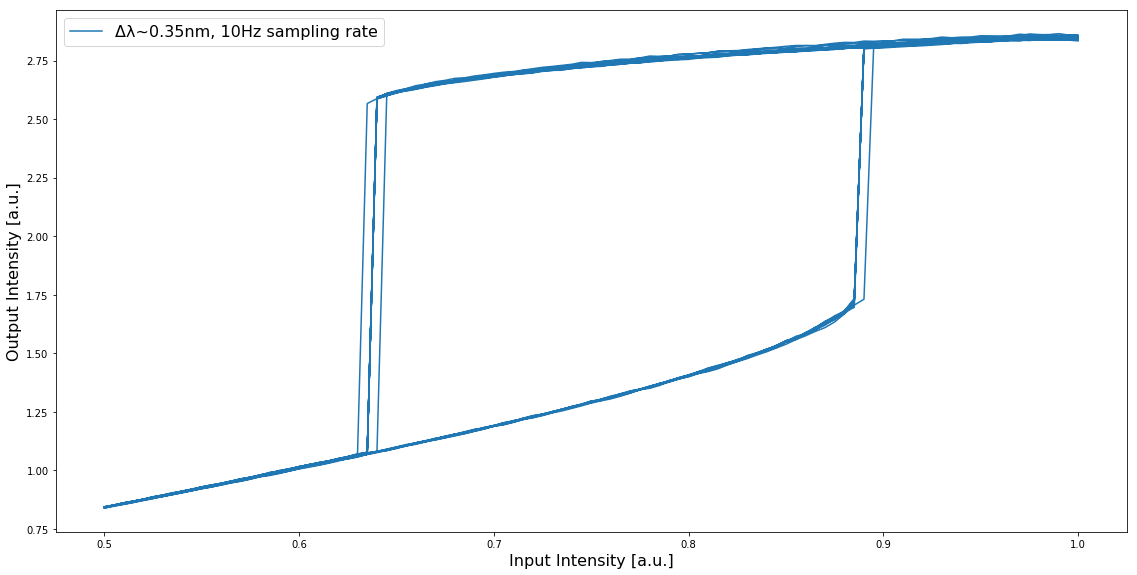
\includegraphics[draft,width=9cm,height=6cm]{figures/foo.png}
	\caption{image/scheme of the minimatrix}
	\label{fig:minimatrix_full}
\end{figure}

\section{The setup}

\section{Results}